%%%%%%%%%%%%%%%%%%%%%%%%%%%%%%%%%%%%%%%%%
% Medium Length Professional CV
% LaTeX Template
% Version 3.0 (December 17, 2022)
%
% This template originates from:
% https://www.LaTeXTemplates.com
%
% Author:
% Vel (vel@latextemplates.com)
%
% Original author:
% Trey Hunner (http://www.treyhunner.com/)
%
% License:
% CC BY-NC-SA 4.0 (https://creativecommons.org/licenses/by-nc-sa/4.0/)
%
%%%%%%%%%%%%%%%%%%%%%%%%%%%%%%%%%%%%%%%%%

%----------------------------------------------------------------------------------------
%	PACKAGES AND OTHER DOCUMENT CONFIGURATIONS
%----------------------------------------------------------------------------------------

\documentclass[
	%a4paper, % Uncomment for A4 paper size (default is US letter)
	11pt, % Default font size, can use 10pt, 11pt or 12pt
]{resume} % Use the resume class

\usepackage{ebgaramond} % Use the EB Garamond font
\usepackage{kotex}
%------------------------------------------------

\name{Wonseo Choi} % Your name to appear at the top

% You can use the \address command up to 3 times for 3 different addresses or pieces of contact information
% Any new lines (\\) you use in the \address commands will be converted to symbols, so each address will appear as a single line.


\address{Seoul, Republic of Korea} % Main address

% \address{123 Pleasant Lane \\ City, State 12345} % A secondary address (optional)

\address{1202won@naver.com} % Contact information
\address{https://wonseo-c.github.io/}

%----------------------------------------------------------------------------------------

\begin{document}


\begin{figure}[h!]
    \centerline{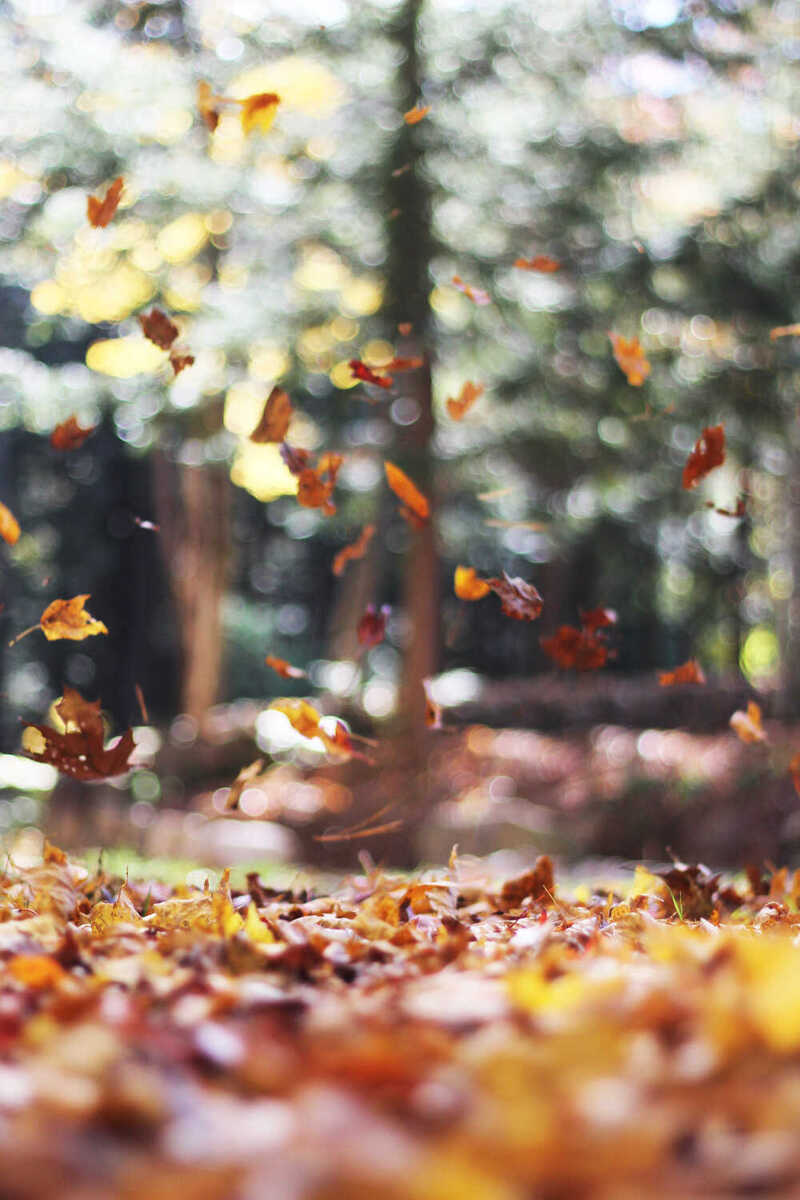
\includegraphics[width=0.33\columnwidth]{../../img/2.jpg}}
  \end{figure}

%----------------------------------------------------------------------------------------
%	EDUCATION SECTION
%----------------------------------------------------------------------------------------

\begin{rSection}{Education}
	\begin{rSubsection}{Hanyang University}{Mar 2022 - Feb 2024}{Master of Science in Electronic Engineering}{}
		\item \textit{Research Topic: AI for Network/Embedded Systems and Modeling/Simulation of Cyber-Physical Systems}
		\item \textit{Overall GPA: 4.44 / 4.5}
	\end{rSubsection}

	\begin{rSubsection}{Hanyang University}{Mar 2017 - Feb 2022}{Bachelor of Science in Electric Engineering}{}
		\item \textit{Minor in Electronic Engineering}
		\item \textit{Overall GPA: 4.07 / 4.5 (Major GPA: 4.18 / 4.5)}
	\end{rSubsection}

\end{rSection}

%----------------------------------------------------------------------------------------
%	PROJECT SECTION
%----------------------------------------------------------------------------------------

\begin{rSection}{reserach project}
	\begin{rSubsection}{AI for Network/Embedded Systems}{}{}{}
		\item Localize WiFi Access Points using Convolutional Neural Network (with KT)
		\item Predict Path-Loss using Deep Neural Network
	
	\end{rSubsection}

	\begin{rSubsection}{Modeling/Simulation of Cyber-Physical Systems}{}{}{}
		\item Support Mutation in Lingua Franca by Implementing Savina Benchmark (with U.C. Berkeley)
	\end{rSubsection}

	
	\begin{rSubsection}{Additional Proejcts}{}{}{}
		\item Fuse IMU Sensors for Location Tracking using Kalman Filter (MCU Board)
		\item Develop Android App for Handwriting Number Recognition using Google ML Kit
		\item Develop Apple Watch App Integrating UWB Technology and Advanced Medical Data Monitoring
		\item Design Localization System using IMU Tag
	\end{rSubsection}
\end{rSection}

%----------------------------------------------------------------------------------------
%	PAPER
%----------------------------------------------------------------------------------------


\begin{rSection}{Paper}

	1. \textbf{W. Choi} et al., "Enhanced Wi-Fi Access Point Positioning Using Hexagonal CNN With Mobile Data and Urban Information," in IEEE Internet of Things Journal, vol. 11, no. 20, pp. 33820-33832, 15 Oct.15, 2024.

	2. Sung, S., \textbf{Choi, W.}, Kim, H., \& Jung, J. I. (2023). Deep Learning-Based Path Loss Prediction for Fifth-Generation New Radio Vehicle Communications. IEEE Access.
	
	3. Kim, T. M., \textbf{Choi, W.}, Choi, I. Y., Park, S. J., Yoon, K. H., \& Chang, D. J. (2021). Semi-AI and Full-AI digitizer: the ways to digitalize visual field big data. Computer Methods and Programs in Biomedicine, 207, 106168.

	4. Suh, S., Cheon, S., \textbf{Choi, W.}, Chung, Y. W., Cho, W. K., Paik, J. S., ... , \& Lee, Y. O. (2022). Supervised segmentation with domain adaptation for small sampled orbital CT images. Journal of Computational Design and Engineering, 9(2), 783-792.

	% \textbf{Thesis for the Master of Science} \\
	% Enhanced Wi-Fi Acess Point Positioning based on Hexagonal CNN using Mobile Measurement and Building/Road Information

\end{rSection}

%----------------------------------------------------------------------------------------
%	WORK EXPERIENCE SECTION
%----------------------------------------------------------------------------------------

\begin{rSection}{Experience}
	\begin{rSubsection}{LG Display}{Mar 2024 - Current}{Big Data Scientist/Engineer}{Paju, Gyeonggi-do}
		\item Analyze big data to improve yield.
		\item Develop R/Python code for Big data processing
	\end{rSubsection}
	
	\begin{rSubsection}{Catholic Univ. of Korea Yeouido ST. Mary's Hospital}{Aug 2020 - Feb 2021}{Research Intern}{Seoul, Korea} 
		\item Develop an automated AI system to extract test results from image-based result sheets using Big Data Processing techniques for AI applications.
		\item Perform experiments and implement research on domain adaptation through Generative Adversarial Networks (GANs).
	\end{rSubsection}
	
	\begin{rSubsection}{KIST Europe}{Feb 2020 - Jul 2020}{Intern}{Saarbrücken, Germany}
		\item Develop an automated AI system to acquire experimental data, enabling heart rate calculation by analyzing size variations of heart images across frames.
		\item Enhance cell tracking performance by optimizing the U-Net layer and analyzing the Localization component for accurate cell tracking.
	\end{rSubsection}

\end{rSection}

%----------------------------------------------------------------------------------------
%	TECHNICAL STRENGTHS SECTION
%----------------------------------------------------------------------------------------

\begin{rSection}{Technical Strengths}

	\begin{tabular}{@{} >{\bfseries}l @{\hspace{6ex}} l @{}}
		Computer Languages & Python(with PyTorch, Tensorflow, Keras), R, MATLAB, Assembly \\
		& Java, C++, TypeScript \\
		\\
		Developing Environments & Mac, Windows, Linux (Ubuntu Server)
	\end{tabular}

\end{rSection}


\begin{rSection}{Graduate Porject}
	
	1. Detect Kickboard with Embedded Hardware (Jetson Nano Board) 

	2. Untact-kiosk: Design and develop a touchless keyboard and mouse using AI detection and clustering.

\end{rSection}

\begin{rSection}{Online-Demo}
	
	\textbf{Wonseo Choi}, Yongoh Lee, “Attention-aware U-Net toward the interpretability of single cell segmentation”, KCCV 2020, Republic of Korea (Online) - demo video
	\\
	\\
\end{rSection}

% \begin{rSection}{Patents}
	
% 	1. Yongoh Lee, Youngjun Kim, Baeckkyeong Sung, Changsun Ryu, Jihoon Park, Jayoung Park, Sungho Suh, \textbf{Wonseo Choi}, Taegeol Lee, Ikhwan Kwon "Method and apparatus for non-invasive real-time monitoring of behavior patterns of ecological species for ecotoxicity risk assessment", KR-Application No. 10-2020-0115178

% 	2. Yunsang Cho, \textbf{Wonseo Choi} “Federate learning system for generative adversarial network”, KR-Application (ongoing)

% \end{rSection}

\begin{rSection}{Other Activities}

	\begin{rSubsection}{겨자씨 키움센터}{Feb 2021 - Aug 2021}{Founding Activities}{}
		\item Obligatory recording paper Digitization Artificial intelligence learning model (module) development
	\end{rSubsection}

	\begin{rSubsection}{Visiting U.C. Berkeley}{Jun 2022 - Jul 2022 , Feb 2023}{}{}
		\item Design and develop the implementation of Lingua-Franca mutations
	\end{rSubsection}

\end{rSection}

\begin{rSection}{Teachiing Assistant}

	\begin{rSubsection}{Probability \& Statistics}{Sep 2023-Dec 2023}{}{}
		\item Generating Random Variables based on Probability distributions using MATLAB
	\end{rSubsection}

	\begin{rSubsection}{Computer Network}{Sep 2023-Dec 2023}{}{}
		\item Basic Algorithm for Computer Network using MATLAB
	\end{rSubsection}

\end{rSection}

\begin{rSection}{Awards}

	1. Academic Excellence Award in the Hanyang Univ. graduation ceremony \hfill \textit {Feb 2022}

	2. Encouragement Award in the "HY-Running Pace Maker" Program \hfill \textit {Jan 2022}

\end{rSection}

%----------------------------------------------------------------------------------------

\end{document}
